\section{Functional roles of dynamical patterns}\label{sec:functional_roles_of_dynamical_patterns}

The dynamics that have been studied in this thesis are characterised by three distinct spatiotemporal signatures: gamma-band oscillations, theta-scale rhythmicity, and superdiffusive spatial trajectories. The framework described in \cref{chap:a_unifying_model} from modelling \cref{eq:fns} in a search task aims to unify these signatures as coupled dynamics which provide flexible functional roles in basic computation. In the present section we identify each dynamical pattern with a particular functional role in sampling: local exploitation in gamma oscillations, temporal organisation in theta rhythmicity, and global exploration through $\alpha$-superdiffusion. Using those metrics laid out in \cref{sec:information-theoretic_metrics}, we can precisely identify the functional role and advantages of each dynamical pattern.

\subsection{Gamma oscillations}
At the finest spatiotemporal scales, both FNS dynamics and empirical gaze dynamics are characterised by high-frequency stochastic local sampling. These dynamics are analogous to the gamma oscillations found throughout the brain in almost every computational task. Within our continuous-time dynamical model, local oscillatory behaviour is controlled by the memory-momentum term $p_t$ and the noise driven by $\alpha$-Lévy noise $dL_t^{\alpha}$ within a highly localised potential well.

From an abstract sampling perspective such local oscillations are related to rapid decorrelation of sampled locations, and regular probing of local gradients in the posterior distribution $\pi_t(\textbf{x})$. In the context of visual sampling, this gradient-awareness is associated with contrast and high spatial frequencies, where ocular microtremor has been shown to be beneficial in perception of high spatial frequencies.


The primary functional role of this gamma-scale activity is to continuously probe the local gradient of the posterior belief distribution, $\pi_t(\textbf{x})$. By oscillating rapidly within a confined neighbourhood, the visual system samples local spatial variations in saliency, thereby rendering the search process robust and responsive to the target landscape $V_t(\textbf{x})$. Furthermore, this dynamic momentum allows for a highly responsive reaction to real-time changes in the saliency landscape. As information is rapidly gathered and the kernel incrementally updates the local landscape, local harmonic oscillations enforce sensitivity to gradients of posterior belief distribution $\pi_t$. The important metrics here are the $IV$, $\frac{dIG}{dH}$, and $FPT$.

\begin{figure}[htbp]
    \centering
    \begin{subfigure}[b]{0.33\textwidth}
        \centering
        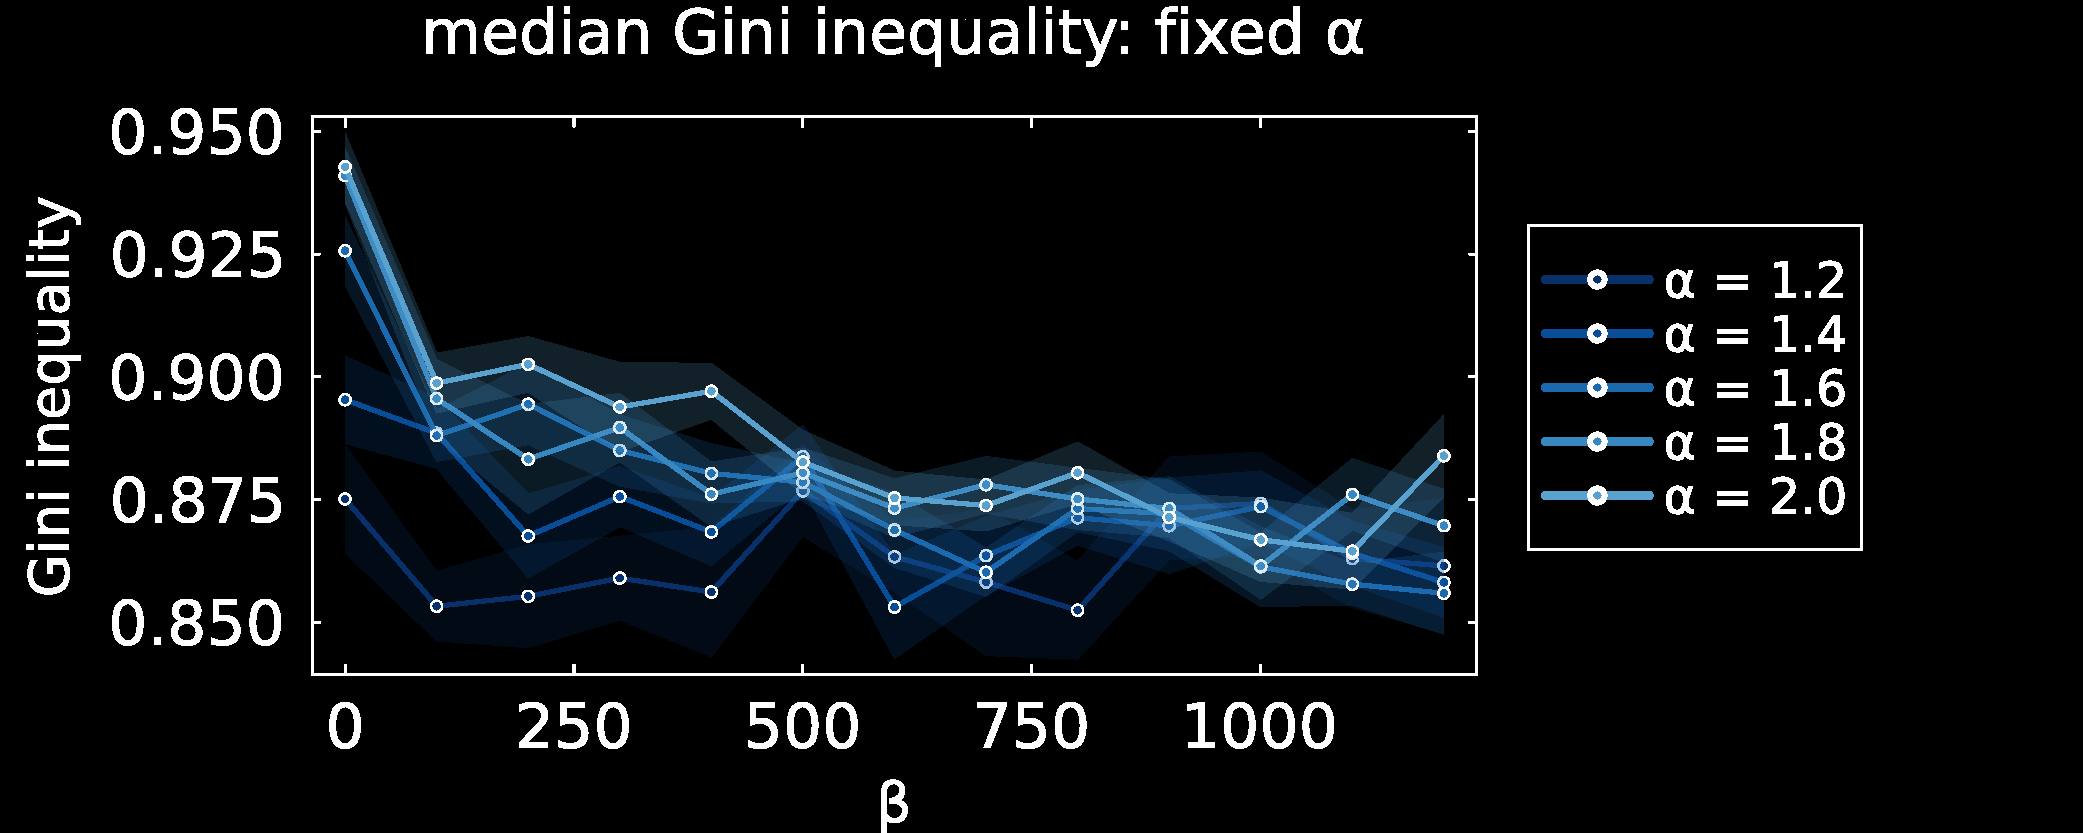
\includegraphics[width=\linewidth]{figures/information_metrics/median_gini_vs_beta.pdf}
        % \caption{\textbf{Rate-corrected rhythmicity index (RCRI) is positively correlated with saccade rate.} Collaborators \textcite{naher_primate_saccades} uncovered this statistically significant result, which implies that shorter inter-saccadic intervals (ISIs) will result in more regular ISIs, which corresponds to stronger kernel dynamics as defined in \cref{sec:adaptive_kernel}.}
        \label{fig:sub1}
    \end{subfigure}
    \vfill
    \begin{subfigure}[b]{0.33\textwidth}
        \centering
        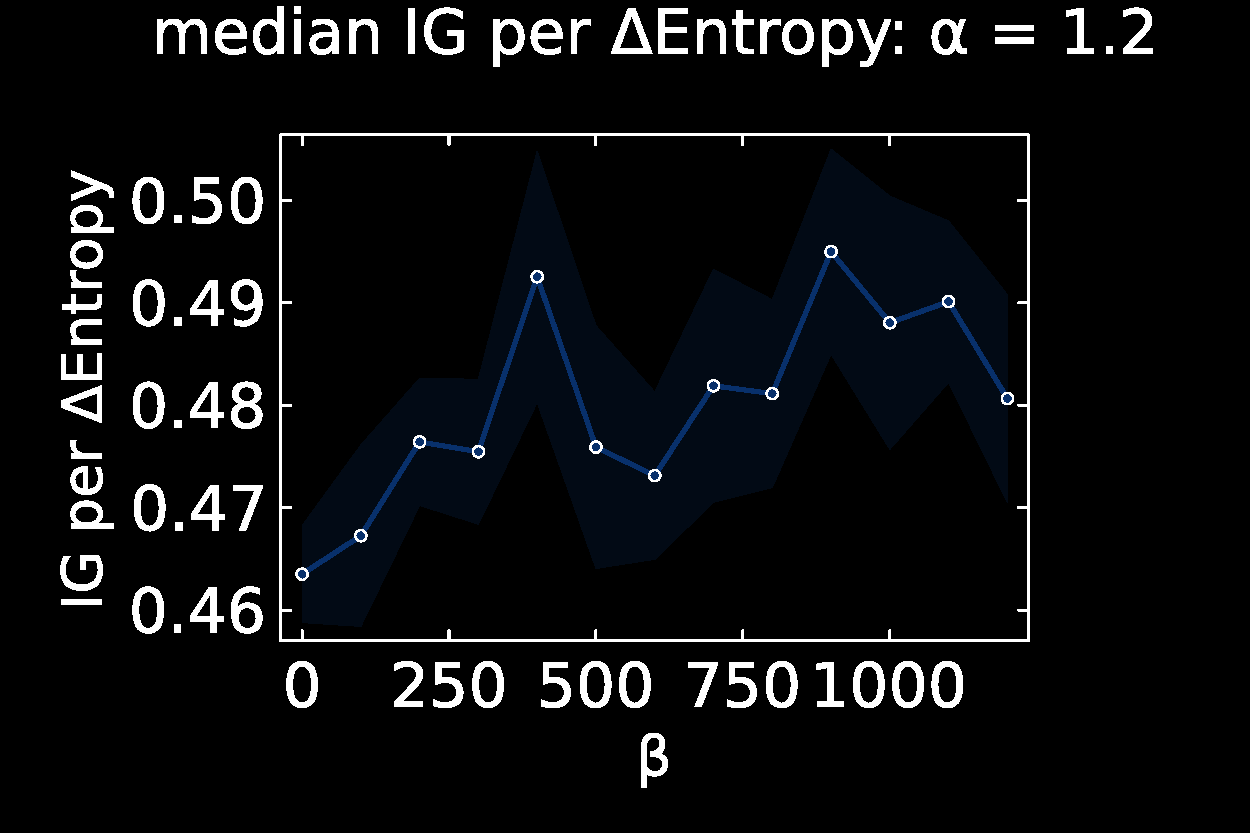
\includegraphics[width=\linewidth]{figures/information_metrics/median_ig_per_dent_alpha1p2_vs_beta.pdf}
        % \caption{\textbf{The probability distribution of inter-saccadic intervals (ISIs) are tightly distributed in a Gamma-10 distribution.} Our collaborators in \textcite{naher_primate_saccades} find that saccades are more locally rhythmic than previously considered. In particular, the ISI distribution is a tight Gamma-10 distribution, but the ISI timeseries is strongly locally rhythmic, as captured by the rate-corrected rhythmicity index (RCRI).}
        \label{fig:sub2}
    \end{subfigure}
    \vfill
    \begin{subfigure}[b]{0.33\textwidth}
        \centering
        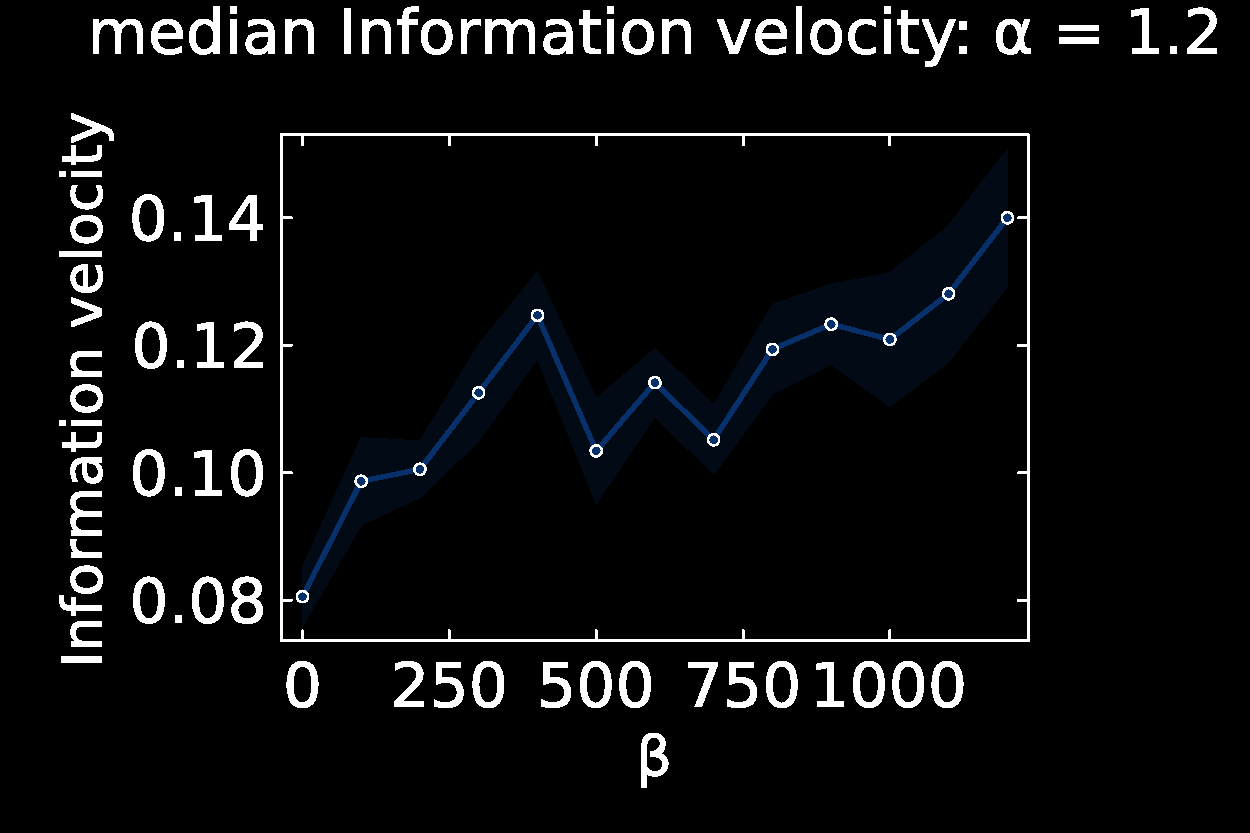
\includegraphics[width=\linewidth]{figures/information_metrics/median_mean_info_velocity_alpha1p2_vs_beta.pdf}
        % \caption{\textbf{The probability distribution of inter-saccadic intervals (ISIs) are tightly distributed in a Gamma-10 distribution.} Our collaborators in \textcite{naher_primate_saccades} find that saccades are more locally rhythmic than previously considered. In particular, the ISI distribution is a tight Gamma-10 distribution, but the ISI timeseries is strongly locally rhythmic, as captured by the rate-corrected rhythmicity index (RCRI).}
        \label{fig:sub2}
    \end{subfigure}
    \vfill
    \begin{subfigure}[b]{0.33\textwidth}
        \centering
        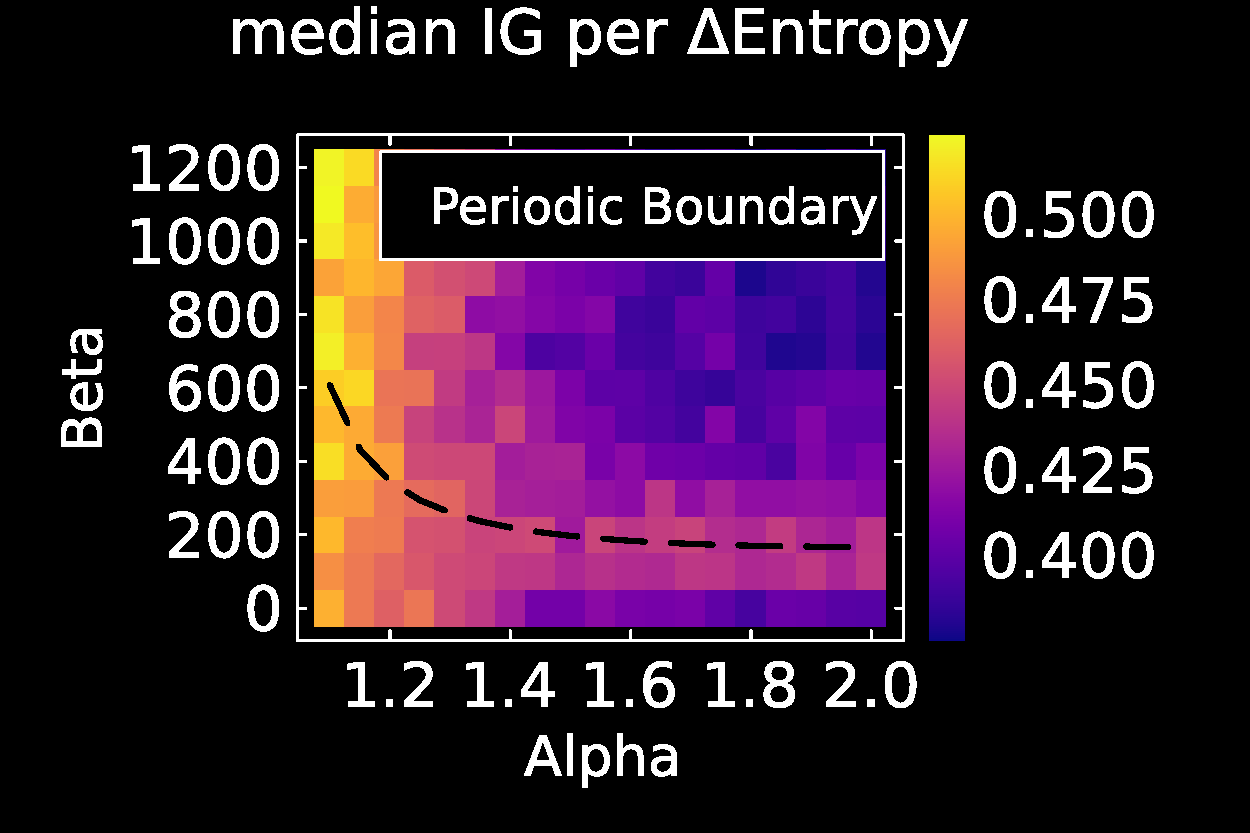
\includegraphics[width=\linewidth]{figures/information_metrics/median_ig_per_dent_heatmap.pdf}
        % \caption{\textbf{The probability distribution of inter-saccadic intervals (ISIs) are tightly distributed in a Gamma-10 distribution.} Our collaborators in \textcite{naher_primate_saccades} find that saccades are more locally rhythmic than previously considered. In particular, the ISI distribution is a tight Gamma-10 distribution, but the ISI timeseries is strongly locally rhythmic, as captured by the rate-corrected rhythmicity index (RCRI).}
        \label{fig:sub2}
    \end{subfigure}
    \vfill
    \begin{subfigure}[b]{0.33\textwidth}
        \centering
        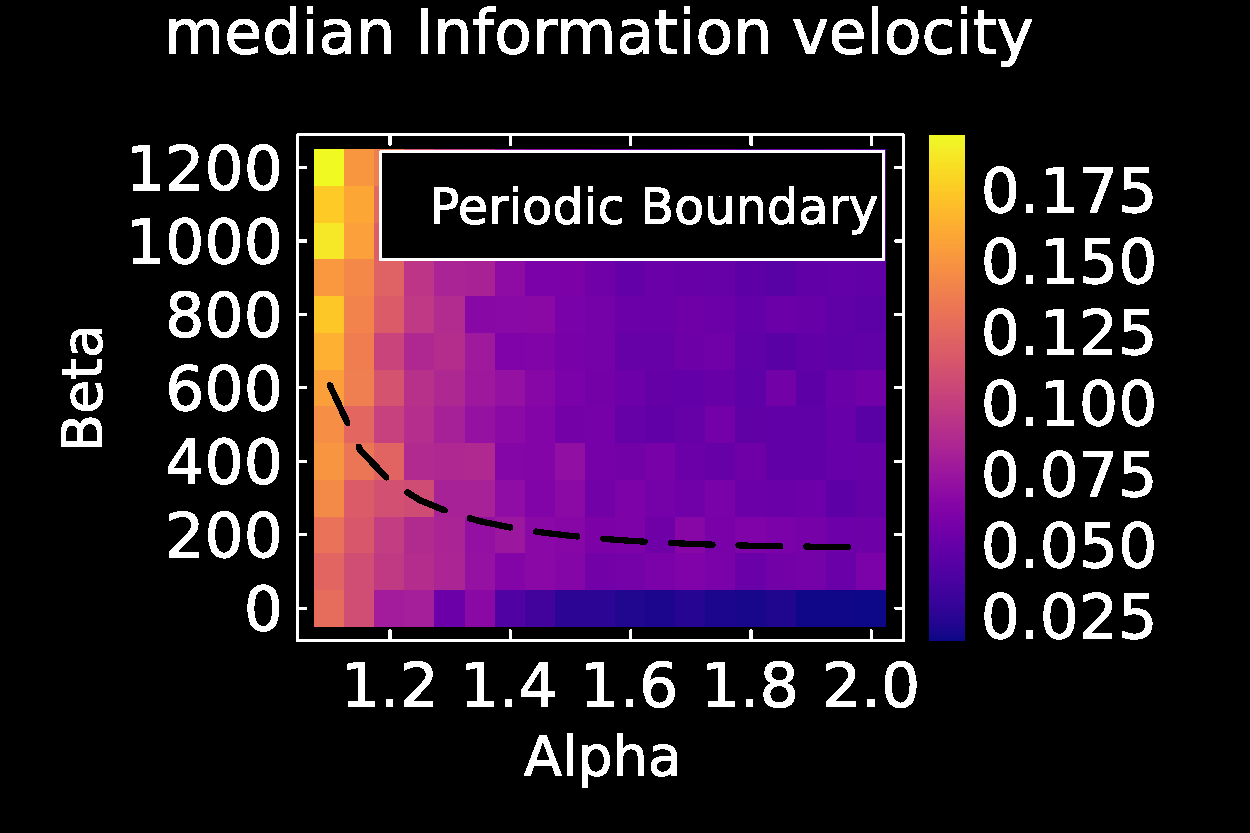
\includegraphics[width=\linewidth]{figures/information_metrics/median_mean_info_velocity_heatmap.pdf}
        % \caption{\textbf{The probability distribution of inter-saccadic intervals (ISIs) are tightly distributed in a Gamma-10 distribution.} Our collaborators in \textcite{naher_primate_saccades} find that saccades are more locally rhythmic than previously considered. In particular, the ISI distribution is a tight Gamma-10 distribution, but the ISI timeseries is strongly locally rhythmic, as captured by the rate-corrected rhythmicity index (RCRI).}
        \label{fig:sub2}
    \end{subfigure}
    \caption{Main figure caption encompassing both subfigures.}
    \label{fig:main}
\end{figure}

\subsection{Theta rhythmicity}
Noise and harmonic neural adaptation dynamics drive local sampling of potential wells, however these periods of local sampling are organised by transitions between sparse areas of high likelihood. Through motion driven by either Lévy- or Brownian noise, transition intervals are exponentially distributed according to a Poisson point process. This is a result of the Lévy-Itô decomposition theorem as presented in \cref{subsec:levy_motion}, where jumps the size of the distance between wells will be Poisson-distributed. However, driving these modal transitions as regular theta-rhythmic events tied to the rate of information acquisition will organise local sampling dynamics to drive higher equality in the amount of information gathered through a cycle of modal exploration.

When testing the effect of theta rhythmic transitions, it is important to examine the dimensionless search effects of varying $\tau$, as $\tau$ directly effects the timescale of information gathering and thus metrics such as $IV$ or $FPT$ will be trivially improved by a decrease in $\tau$.


\subsection{Superdiffusion}
The final dynamical search strategy is superdiffusion, allowing spatially global exploration. Superdiffusive search paths are thought to be optimal when exploring sparse unknown landscapes under the Lévy foraging hypothesis, as described in \cref{subsubsec:anomalous_superdiffusion}. Here, superdiffusion governs the spatial scaling of global exploration, where temporal dynamics of rhythmically organised local sampling of potential wells are explored globally, with superdiffusion allowing long range access to unknown information. 

Scale-free spatial exploration allows the model to rapidly traverse expanses of low-likelihood space. Ultimately, the superdiffusive parameter $\alpha$ is the structural mechanism that prevents the sampler from becoming permanently trapped in a locally depleted belief minimum, ensuring global convergence of the visual inference task. 

\begin{figure}[htbp]
    \centering
    \begin{subfigure}[b]{0.33\textwidth}
        \centering
        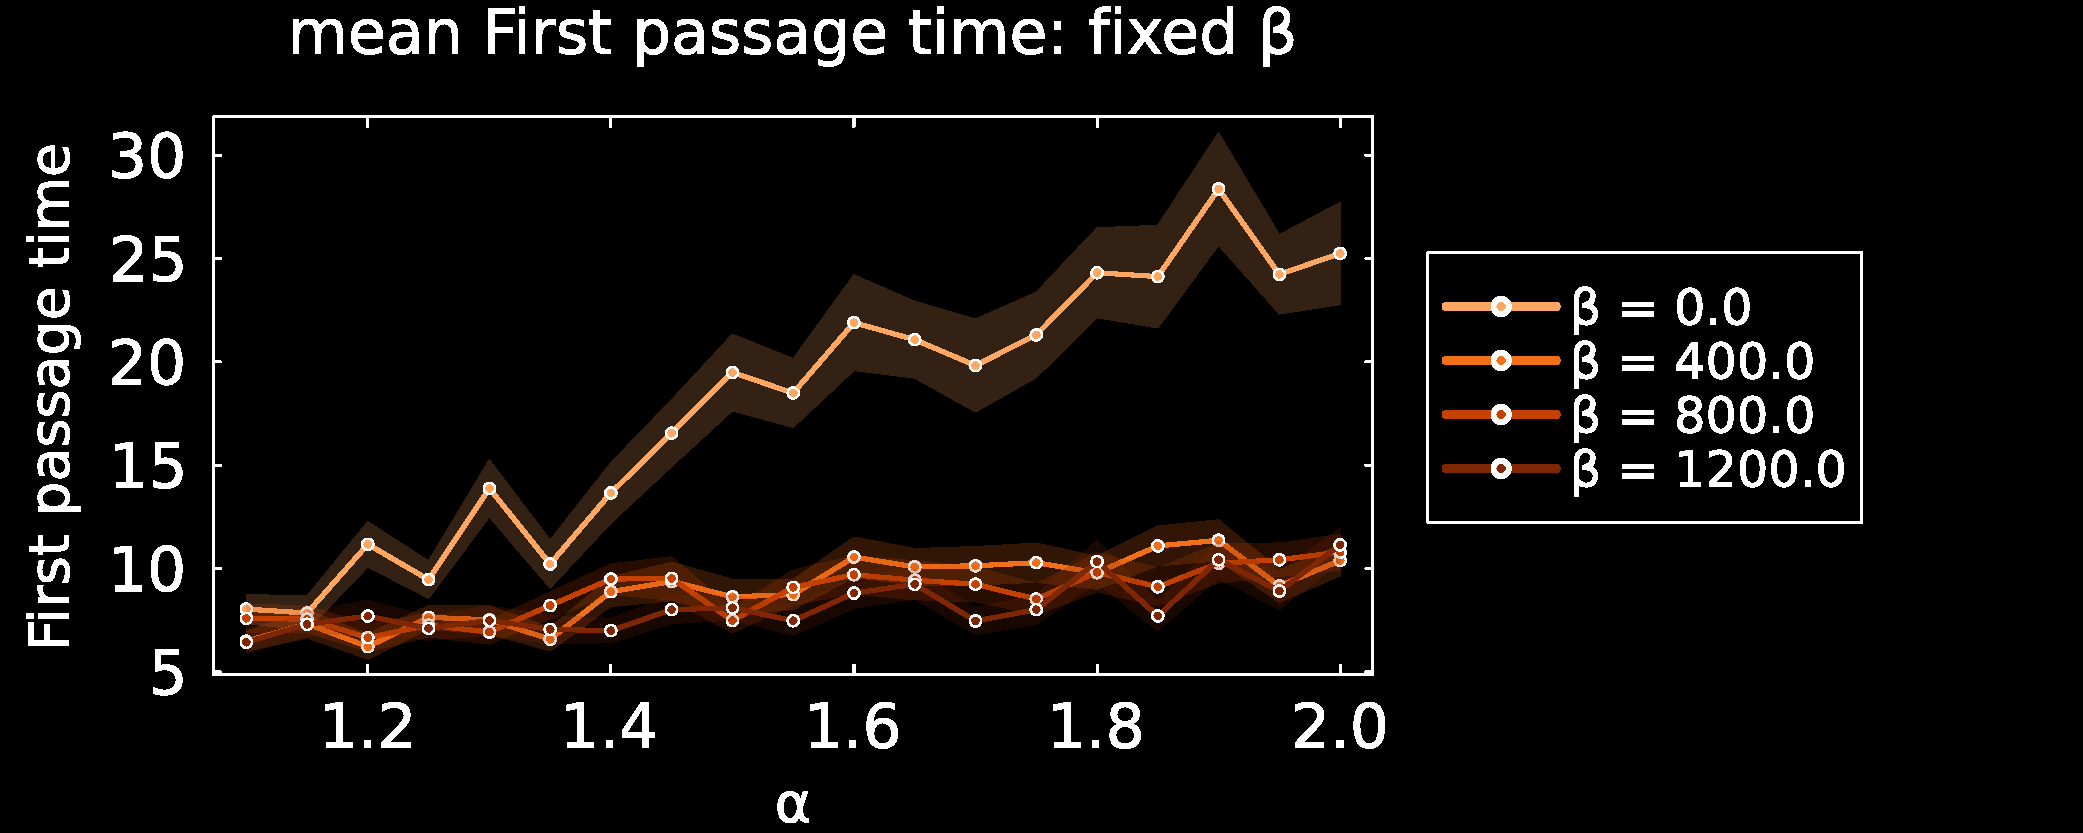
\includegraphics[width=\linewidth]{figures/information_metrics/mean_fpt_vs_alpha.pdf}
        % \caption{\textbf{Rate-corrected rhythmicity index (RCRI) is positively correlated with saccade rate.} Collaborators \textcite{naher_primate_saccades} uncovered this statistically significant result, which implies that shorter inter-saccadic intervals (ISIs) will result in more regular ISIs, which corresponds to stronger kernel dynamics as defined in \cref{sec:adaptive_kernel}.}
        \label{fig:sub1}
    \end{subfigure}
    \vfill
    \begin{subfigure}[b]{0.33\textwidth}
        \centering
        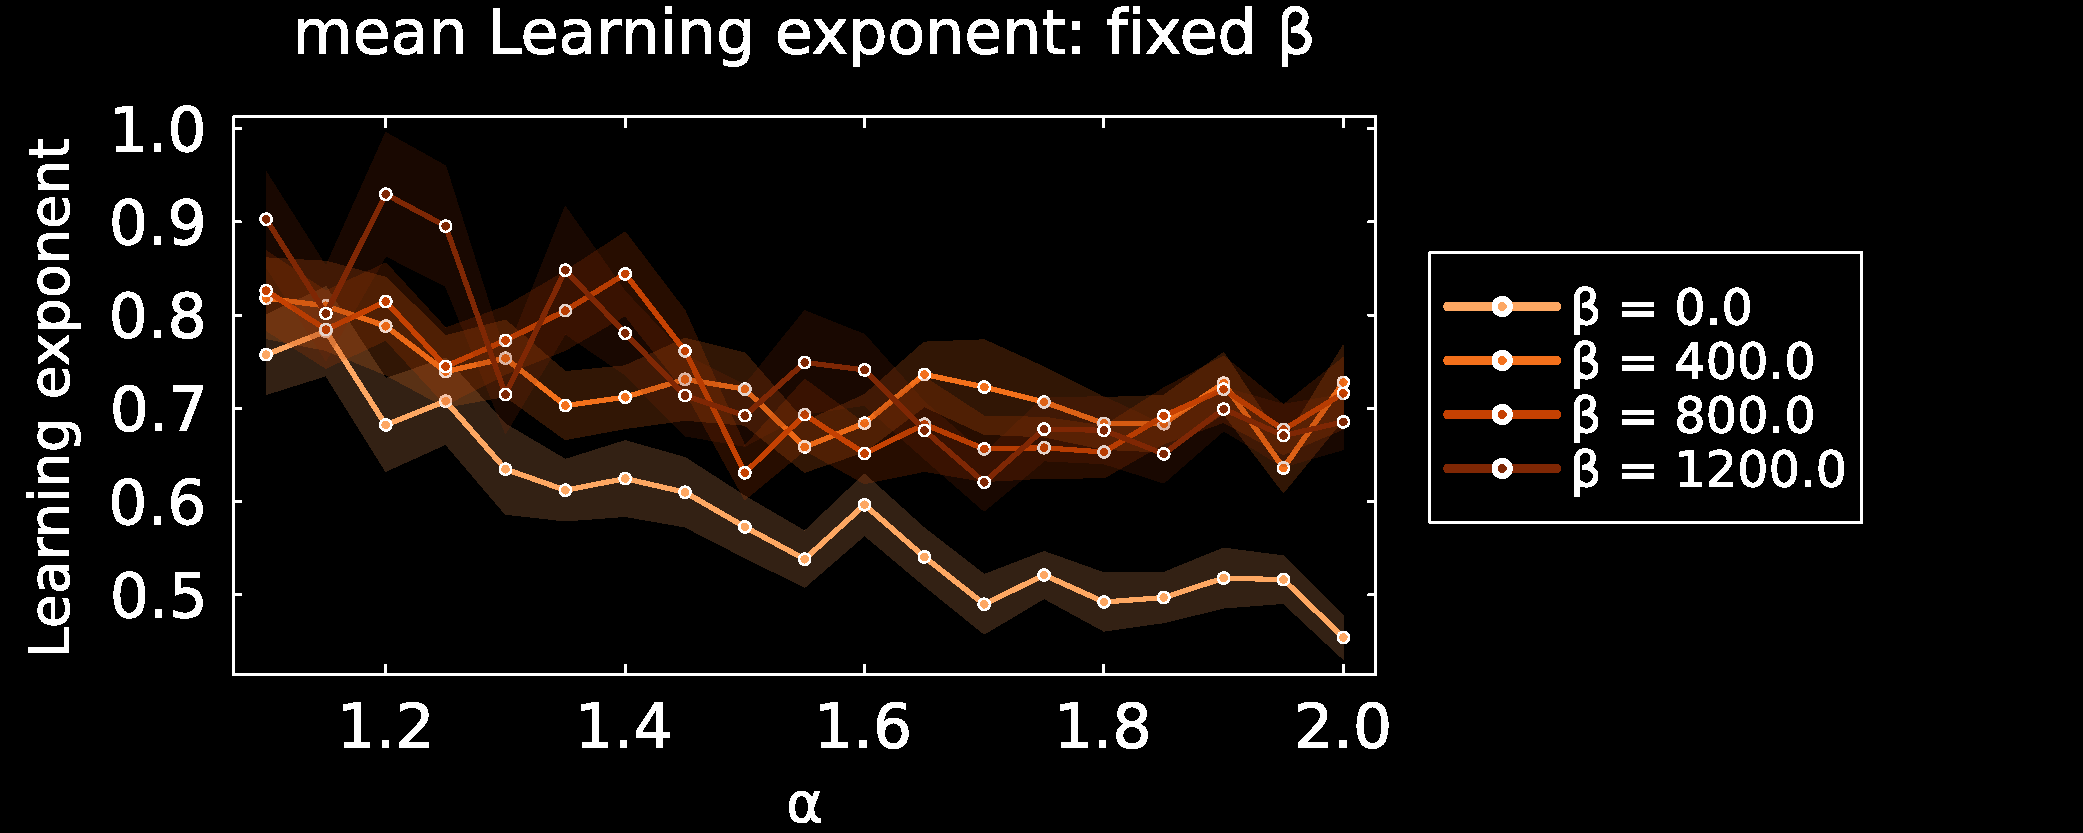
\includegraphics[width=\linewidth]{figures/information_metrics/mean_exponent_shape_vs_alpha.pdf}
        % \caption{\textbf{The probability distribution of inter-saccadic intervals (ISIs) are tightly distributed in a Gamma-10 distribution.} Our collaborators in \textcite{naher_primate_saccades} find that saccades are more locally rhythmic than previously considered. In particular, the ISI distribution is a tight Gamma-10 distribution, but the ISI timeseries is strongly locally rhythmic, as captured by the rate-corrected rhythmicity index (RCRI).}
        \label{fig:sub2}
    \end{subfigure}
    \vfill
    \begin{subfigure}[b]{0.33\textwidth}
        \centering
        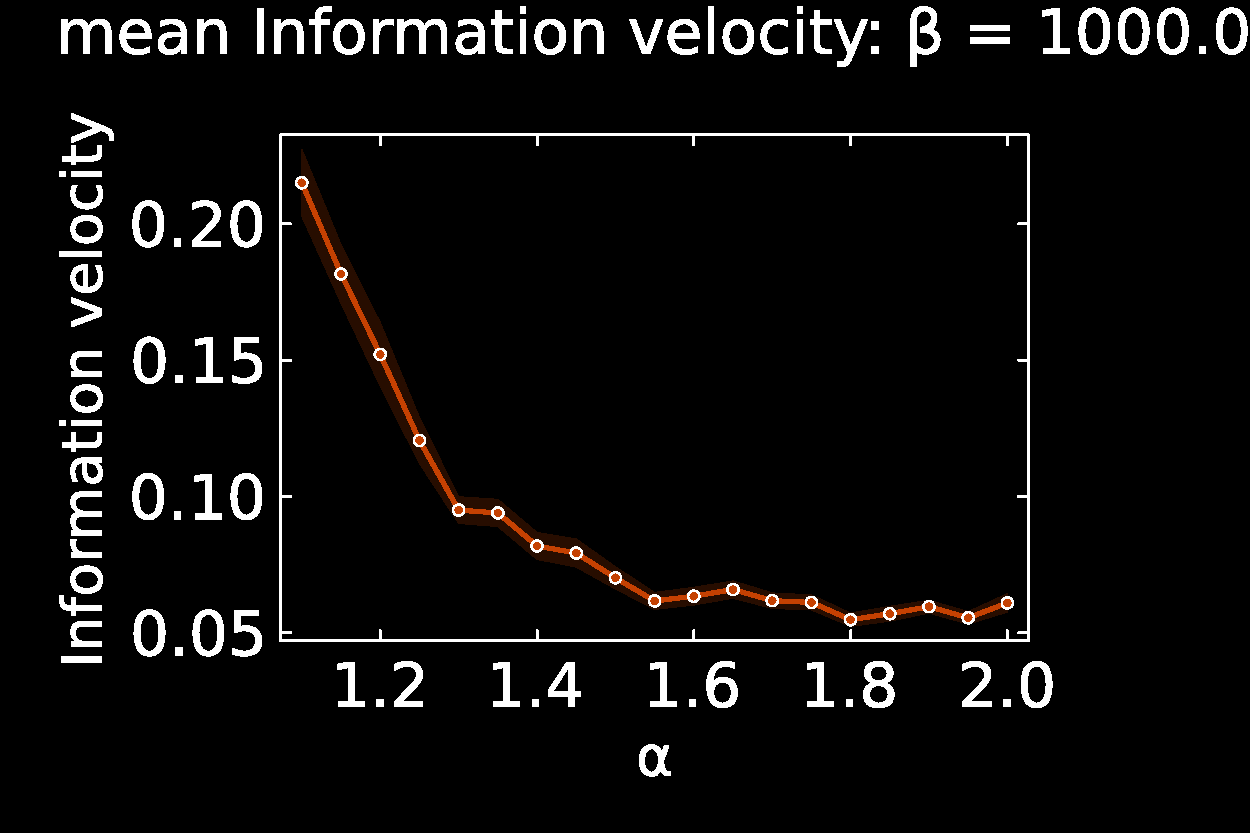
\includegraphics[width=\linewidth]{figures/information_metrics/mean_mean_info_velocity_beta1000_vs_alpha.pdf}
        % \caption{\textbf{The probability distribution of inter-saccadic intervals (ISIs) are tightly distributed in a Gamma-10 distribution.} Our collaborators in \textcite{naher_primate_saccades} find that saccades are more locally rhythmic than previously considered. In particular, the ISI distribution is a tight Gamma-10 distribution, but the ISI timeseries is strongly locally rhythmic, as captured by the rate-corrected rhythmicity index (RCRI).}
        \label{fig:sub2}
    \end{subfigure}
    \vfill
    \begin{subfigure}[b]{0.33\textwidth}
        \centering
        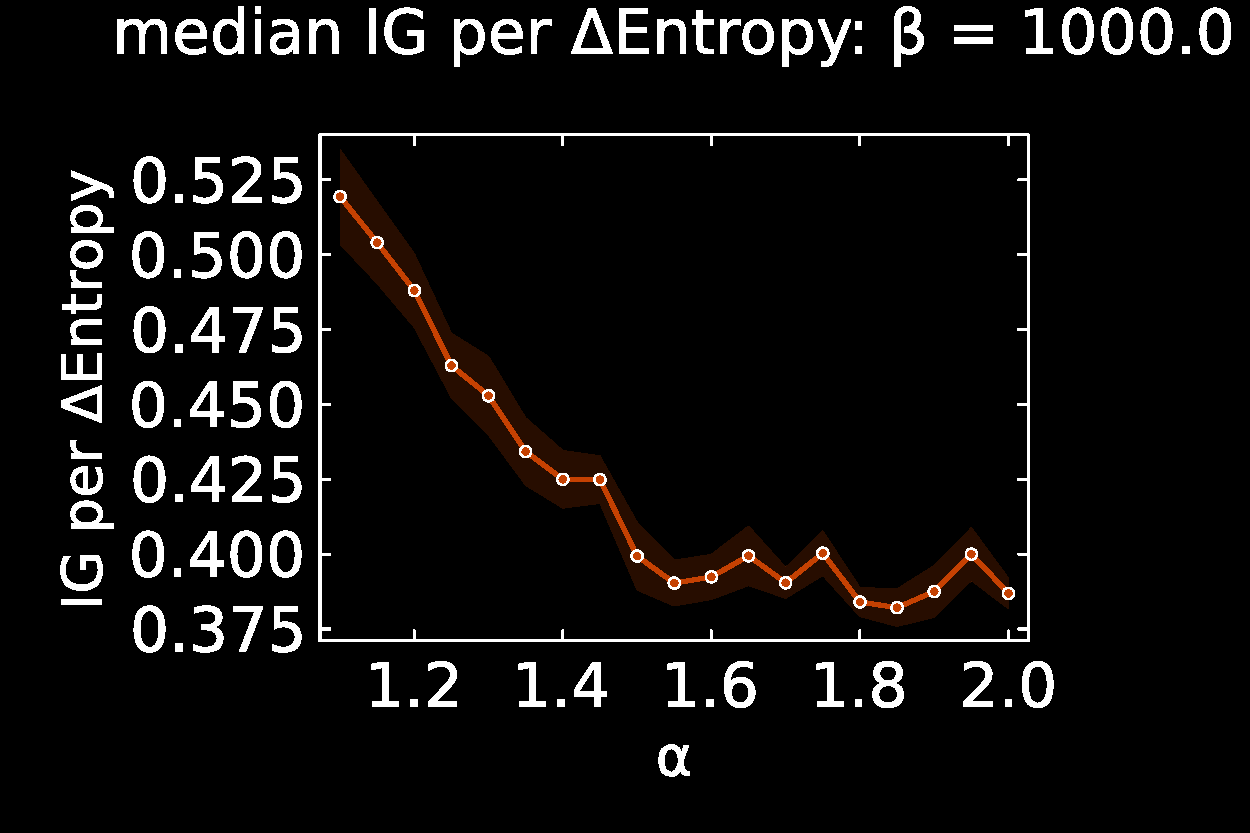
\includegraphics[width=\linewidth]{figures/information_metrics/median_ig_per_dent_beta1000_vs_alpha.pdf}
        % \caption{\textbf{The probability distribution of inter-saccadic intervals (ISIs) are tightly distributed in a Gamma-10 distribution.} Our collaborators in \textcite{naher_primate_saccades} find that saccades are more locally rhythmic than previously considered. In particular, the ISI distribution is a tight Gamma-10 distribution, but the ISI timeseries is strongly locally rhythmic, as captured by the rate-corrected rhythmicity index (RCRI).}
        \label{fig:sub2}
    \end{subfigure}
    \caption{Main figure caption encompassing both subfigures.}
    \label{fig:main}
\end{figure}